% questions.tex —— 1988 年·全国卷·文科 · 题目内容片段（无答案）
% 由 tools/generate_projects.py 依来源总账自 1988/1988_数学真题_全国文_试题.md 生成，勿手改（改源 MD 后重跑）


\gkpart{文科数学}

\begin{gktip}
\textbf{来源说明}：本题面依据固定源 PDF《1988 普通高等学校招生考试（全国卷文）》逐题转录。固定源共 1 页、原卷印刷页码 33；PDF 含题面文字层和矢量图形，但不含答案、解析或评分标准，以下答案和解析由本库独立推导。

\textbf{图形说明}：第 4、12、22 题的函数图象、正四棱台和四棱锥图依据固定源图形关系重绘为 TikZ 矢量图。
\end{gktip}

\begin{question}
\gkti{1}复数

\nopagebreak[4]
\[
\left(\frac{1-i}{1+i}\right)^2
\]

的值等于\mbox{（　　）}

（A）$1$　　（B）$-1$　　（C）$i$　　（D）$-i$

\end{question}
\begin{question}
\gkti{2}圆 $M$ 的方程为

\nopagebreak[4]
\[
(x-3)^2+(y-2)^2=2,
\]

\Needspace{5\baselineskip}
直线 $L$ 的方程为

\nopagebreak[4]
\[
x+y-3=0,
\]

点 $P$ 的坐标为 $(2,1)$，那么\mbox{（　　）}

（A）点 $P$ 在直线 $L$ 上，但不在圆 $M$ 上

（B）点 $P$ 在圆 $M$ 上，但不在直线 $L$ 上

（C）点 $P$ 既在圆 $M$ 上，又在直线 $L$ 上

（D）点 $P$ 既不在直线 $L$ 上，也不在圆 $M$ 上

\end{question}
\begin{question}
\gkti{3}集合 $\{1,2,3\}$ 的子集共有\mbox{（　　）}

（A）5 个　　（B）6 个　　（C）7 个　　（D）8 个

\Needspace{0.4\textheight}
\end{question}
\begin{question}
\gkti{4}函数

\nopagebreak[4]
\[
y=a^x\qquad(0<a<1)
\]

的图象是\mbox{（　　）}
\nopagebreak[4]
\begin{center}% 1988 年全国卷文科第 4 题：指数函数图象的四个选项
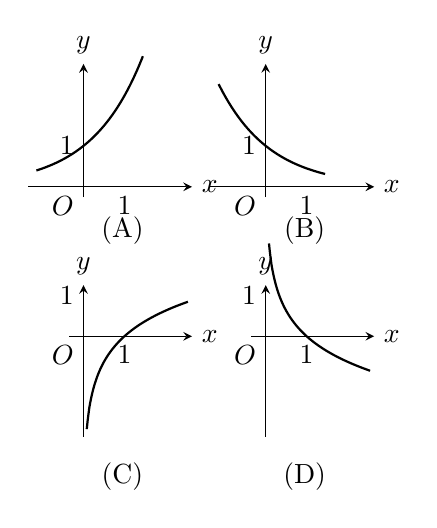
\begin{tikzpicture}[scale=0.52,>=stealth]
  \begin{scope}
    \draw[->] (-1.35,0)--(2.65,0) node[right] {$x$};
    \draw[->] (0,-0.25)--(0,3.0) node[above] {$y$};
    \draw[thick,domain=-1.15:1.45,samples=100]
      plot (\x,{exp(0.8*\x)});
    \node[left] at (0,1) {$1$};
    \node[below] at (1,0) {$1$};
    \node[below left] at (0,0) {$O$};
    \node[below] at (0.95,-0.5) {(A)};
  \end{scope}

  \begin{scope}[xshift=4.45cm]
    \draw[->] (-1.35,0)--(2.65,0) node[right] {$x$};
    \draw[->] (0,-0.25)--(0,3.0) node[above] {$y$};
    \draw[thick,domain=-1.15:1.45,samples=100]
      plot (\x,{exp(-0.8*\x)});
    \node[left] at (0,1) {$1$};
    \node[below] at (1,0) {$1$};
    \node[below left] at (0,0) {$O$};
    \node[below] at (0.95,-0.5) {(B)};
  \end{scope}

  \begin{scope}[yshift=-3.65cm]
    \draw[->] (-0.35,0)--(2.65,0) node[right] {$x$};
    \draw[->] (0,-2.45)--(0,1.25) node[above] {$y$};
    \draw[thick,domain=0.08:2.55,samples=120]
      plot (\x,{0.9*ln(\x)});
    \node[left] at (0,1) {$1$};
    \node[below] at (1,0) {$1$};
    \node[below left] at (0,0) {$O$};
    \node[below] at (0.95,-2.85) {(C)};
  \end{scope}

  \begin{scope}[xshift=4.45cm,yshift=-3.65cm]
    \draw[->] (-0.35,0)--(2.65,0) node[right] {$x$};
    \draw[->] (0,-2.45)--(0,1.25) node[above] {$y$};
    \draw[thick,domain=0.08:2.55,samples=120]
      plot (\x,{-0.9*ln(\x)});
    \node[left] at (0,1) {$1$};
    \node[below] at (1,0) {$1$};
    \node[below left] at (0,0) {$O$};
    \node[below] at (0.95,-2.85) {(D)};
  \end{scope}
\end{tikzpicture}
\end{center}
\nopagebreak[4]
\end{question}
\begin{question}
\gkti{5}已知椭圆方程

\nopagebreak[4]
\[
\frac{x^2}{20}+\frac{y^2}{11}=1,
\]

那么它的焦距是\mbox{（　　）}

（A）$6$　　（B）$3$　　（C）$2\sqrt{31}$　　（D）$\sqrt{31}$

\end{question}
\begin{question}
\gkti{6}在复平面内，与复数

\nopagebreak[4]
\[
z=-1-i
\]

的共轭复数对应的点位于\mbox{（　　）}

（A）第一象限　　（B）第二象限　　（C）第三象限　　（D）第四象限

\end{question}
\begin{question}
\gkti{7}在

\nopagebreak[4]
\[
(x-\sqrt3)^{10}
\]

的展开式中，$x^6$ 的系数是\mbox{（　　）}

（A）$-27C_{10}^{6}$　　（B）$27C_{10}^{4}$

（C）$-9C_{10}^{6}$　　（D）$9C_{10}^{4}$

\end{question}
\begin{question}
\gkti{8}函数

\nopagebreak[4]
\[
y=3\cos\left(\frac25x-\frac\pi6\right)
\]

的最小正周期是\mbox{（　　）}

（A）$\frac25\pi$　　（B）$\frac52\pi$　　（C）$2\pi$　　（D）$5\pi$

\end{question}
\begin{question}
\gkti{9}$\sin\left(-\dfrac{19}{6}\pi\right)$ 的值等于\mbox{（　　）}

（A）$\frac12$　　（B）$-\frac12$　　（C）$\frac{\sqrt3}{2}$　　（D）$-\frac{\sqrt3}{2}$

\end{question}
\begin{question}
\gkti{10}直线

\nopagebreak[4]
\[
x+ay=2a+2
\]

\Needspace{5\baselineskip}
与直线

\nopagebreak[4]
\[
ax+y=a+1
\]

平行（不重合）的充要条件是\mbox{（　　）}

（A）$a=\frac12$　　（B）$a=-\frac12$　　（C）$a=1$　　（D）$a=-1$

\end{question}
\begin{question}
\gkti{11}函数

\nopagebreak[4]
\[
y=\frac{x-2}{2x-1}\qquad\left(x\in R,\ x\ne\frac12\right)
\]

的反函数是\mbox{（　　）}

（A）$y=\frac{x-2}{2x-1}\ (x\in R,\ x\ne\frac12)$

（B）$y=\frac{2x-1}{x-2}\ (x\in R,\ x\ne2)$

（C）$y=\frac{x+2}{2x-1}\ (x\in R,\ x\ne\frac12)$

（D）$y=\frac{2x-1}{x+2}\ (x\in R,\ x\ne-2)$

\Needspace{0.4\textheight}
\end{question}
\begin{question}
\gkti{12}如图，正四棱台中，$A'D'$ 所在的直线与 $BB'$ 所在的直线是\mbox{（　　）}
\nopagebreak[4]
\begin{center}% 1988 年全国卷文科第 12 题：正四棱台
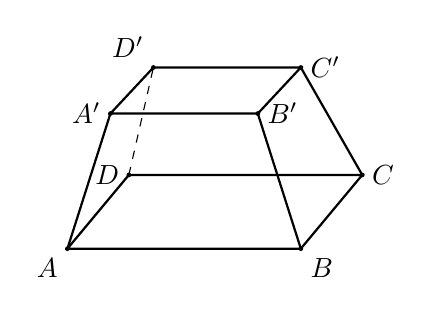
\begin{tikzpicture}[scale=0.78,>=stealth]
  \coordinate (A) at (0,0);
  \coordinate (B) at (3.8,0);
  \coordinate (C) at (4.8,1.2);
  \coordinate (D) at (1.0,1.2);
  \coordinate (Ap) at (0.7,2.2);
  \coordinate (Bp) at (3.1,2.2);
  \coordinate (Cp) at (3.8,2.95);
  \coordinate (Dp) at (1.4,2.95);
  \draw[thick] (A)--(B)--(C)--(D)--cycle;
  \draw[thick] (Ap)--(Bp)--(Cp)--(Dp)--cycle;
  \draw[thick] (A)--(Ap) (B)--(Bp) (C)--(Cp);
  \draw[dashed] (D)--(Dp);
  \fill (A) circle (1.1pt) node[below left] {$A$};
  \fill (B) circle (1.1pt) node[below right] {$B$};
  \fill (C) circle (1.1pt) node[right] {$C$};
  \fill (D) circle (1.1pt) node[left] {$D$};
  \fill (Ap) circle (1.1pt) node[left] {$A'$};
  \fill (Bp) circle (1.1pt) node[right] {$B'$};
  \fill (Cp) circle (1.1pt) node[right] {$C'$};
  \fill (Dp) circle (1.1pt) node[above left] {$D'$};
\end{tikzpicture}
\end{center}
\nopagebreak[4]
（A）相交直线　　（B）平行直线

（C）不互相垂直的异面直线　　（D）互相垂直的异面直线

\end{question}
\begin{question}
\gkti{13}函数

\nopagebreak[4]
\[
y=\sin\left(x+\frac\pi4\right)
\]

在闭区间\mbox{（　　）}上是增函数

（A）$\left[-\frac\pi2,\frac\pi2\right]$　　（B）$\left[-\frac{3\pi}{4},\frac\pi4\right]$

（C）$[-\pi,0]$　　（D）$\left[-\frac\pi4,\frac{3\pi}{4}\right]$

\end{question}
\begin{question}
\gkti{14}假设在 200 件产品中有 3 件次品，现在从中任意抽取 5 件，其中至少有 2 件次品的抽法有\mbox{（　　）}

（A）$C_3^2C_{197}^3+C_3^3C_{197}^2$ 种

（B）$C_3^2C_{197}^3$ 种

（C）$C_{200}^5-C_{197}^5$ 种

（D）$C_{200}^5-C_3^1C_{197}^4$ 种

\end{question}
\begin{question}
\gkti{15}已知二面角 $\alpha-AB-\beta$ 的平面角是锐角 $\theta$，$\alpha$ 内一点 $C$ 到 $\beta$ 的距离为 $3$，点 $C$ 到棱 $AB$ 的距离为 $4$，那么 $\tan\theta$ 的值等于\mbox{（　　）}

（A）$\frac34$　　（B）$\frac35$　　（C）$\frac{3\sqrt7}{7}$　　（D）$\frac{\sqrt7}{3}$

\end{question}
\begin{question}
\gkti{16}求复数

\nopagebreak[4]
\[
\sqrt3-i
\]

的模和辐角的主值。

\end{question}
\begin{question}
\gkti{17}解方程

\nopagebreak[4]
\[
9^{-x}-2\cdot3^{1-x}=27.
\]

\end{question}
\begin{question}
\gkti{18}已知

\nopagebreak[4]
\[
\sin\theta=-\frac35,\qquad
3\pi<\theta<\frac{7\pi}{2},
\]

\Needspace{5\baselineskip}
求

\nopagebreak[4]
\[
\tan\frac\theta2.
\]

\end{question}
\begin{question}
\gkti{19}一个直角三角形的两条直角边的长分别为 $3\text{ cm}$ 和 $4\text{ cm}$，将这个直角三角形以斜边为轴旋转一周，求所得旋转体的体积。

\end{question}
\begin{question}
\gkti{20}求极限

\nopagebreak[4]
\[
\lim_{n\to\infty}\frac{3n^2+2n}{n^2+3n-1}.
\]

\end{question}
\begin{question}
\gkti{21}证明：

\nopagebreak[4]
\[
\cos3\alpha=4\cos^3\alpha-3\cos\alpha.
\]

\Needspace{0.4\textheight}
\end{question}
\begin{question}
\gkti{22}如图，四棱锥 $S-ABCD$ 的底面是边长为 $1$ 的正方形，侧棱 $SB$ 垂直于底面，并且

\nopagebreak[4]
\[
SB=\sqrt3.
\]

用 $\alpha$ 表示 $\angle ASD$，求 $\sin\alpha$。
\nopagebreak[4]
\begin{center}% 1988 年全国卷文科第 22 题：四棱锥 S-ABCD
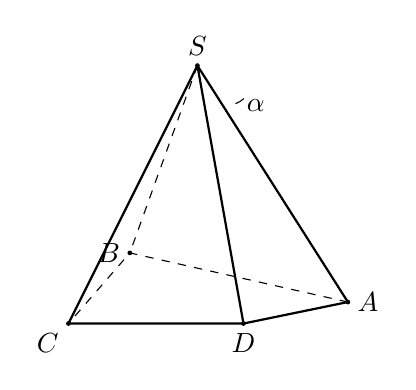
\begin{tikzpicture}[scale=0.78,>=stealth]
  \coordinate (S) at (2.1,4.2);
  \coordinate (B) at (1.0,1.15);
  \coordinate (A) at (4.55,0.35);
  \coordinate (D) at (2.85,0.0);
  \coordinate (C) at (0,0.0);
  \draw[thick] (S)--(C) (S)--(D) (S)--(A);
  \draw[dashed] (S)--(B);
  \draw[thick] (C)--(D)--(A);
  \draw[dashed] (A)--(B)--(C);
  \draw (2.72,3.58) arc (-70:-48:0.42);
  \node at (3.05,3.55) {$\alpha$};
  \fill (S) circle (1.1pt) node[above] {$S$};
  \fill (A) circle (1.1pt) node[right] {$A$};
  \fill (B) circle (1.1pt) node[left] {$B$};
  \fill (C) circle (1.1pt) node[below left] {$C$};
  \fill (D) circle (1.1pt) node[below] {$D$};
\end{tikzpicture}
\end{center}
\nopagebreak[4]
\end{question}
\begin{question}
\gkti{23}在双曲线

\nopagebreak[4]
\[
x^2-y^2=1
\]

的右支上求点 $P(a,b)$，使该点到直线 $y=x$ 的距离为 $\sqrt2$。

\end{question}
\begin{question}
\gkti{24}解不等式：

\nopagebreak[4]
\[
\lg\left(x-\frac1x\right)<0.
\]

\end{question}
\begin{question}
\gkti{25}一个数列 $\{a_n\}$：当 $n$ 为奇数时，

\nopagebreak[4]
\[
a_n=5n+1;
\]

\Needspace{5\baselineskip}
当 $n$ 为偶数时，

\nopagebreak[4]
\[
a_n=2^{n/2}.
\]

求这个数列的前 $2m$ 项的和（$m$ 是正整数）。

\end{question}